%!TEX encoding = UTF-8 Unicode
%!TEX root = ../compendium2.tex

\section{Visual Studio Code med tillägget Scala Metals}\label{appendix:ide:vscode}

Visual Studio Code\footnote{\href{https://en.wikipedia.org/wiki/Visual\_Studio\_Code}{en.wikipedia.org/wiki/Visual\_Studio\_Code}}, förkortat VS Code eller bara \code{code}, är en gratis utvecklingsmiljö som är mestadels öppen källkod\footnote{Varianten VS Codium \url{https://vscodium.com/} är helt fri från stängd källkod och telemetri.}. Projektet startades och leds av Microsoft och har en aktiv gemenskap med många utvecklare och många användbara tillägg \Eng{extensions}.

VS Code kallas ofta för ''bara'' en editor, men har genom åren utvecklats till en fullfjädrad IDE med bl.a. inbyggd debugger och stöd för många olika språk via ett omfattande bibliotek av tillägg.%

\begin{itemize}
\item 
Läs mer om hur man använder VS Code här: \\
\url{https://code.visualstudio.com/docs}

\item
Läs mer om hur du använder Scala i VS Code här: \\
\url{https://scalameta.org/metals/docs/editors/vscode}

\end{itemize}

Det finns många användbara kortkommandon som gör dig snabbare och snabbare när du kodar, allteftersom du lär dig nya kortkommandon. Ett bra tips är att du lär dig minst ett nytt kortkommando om dagen och efter ett tag kan du riktigt många. Här finns en sammanfattning av de viktigaste kortkommandona för VS Code för Linux:\\
\url{https://code.visualstudio.com/shortcuts/keyboard-shortcuts-linux.pdf}\\
Byt ut \code{linux} mot \code{windows} eller \code{macos} i adressen ovan för motsvarande plattform.

\subsection{Installera VS Code och Metals}\label{appendix:ide:vscode:install}

VS Code är förinstallerad på LTH:s datorer, men du behöver själv installera Scala-tillägget \textbf{Metals} första gången du kör igång VS Code på LTH:s datorer. Läs om installation av Metals här: \\
\url{https://marketplace.visualstudio.com/items?itemName=scalameta.metals} 

Läs mer om hur du installerar VS Code på din egen dator här: \\\url{https://code.visualstudio.com}

Mer information om installation av verktyg finns på kursens hemsida: \\
\url{https://cs.lth.se/pgk/verktyg}

\begin{figure}
\centering
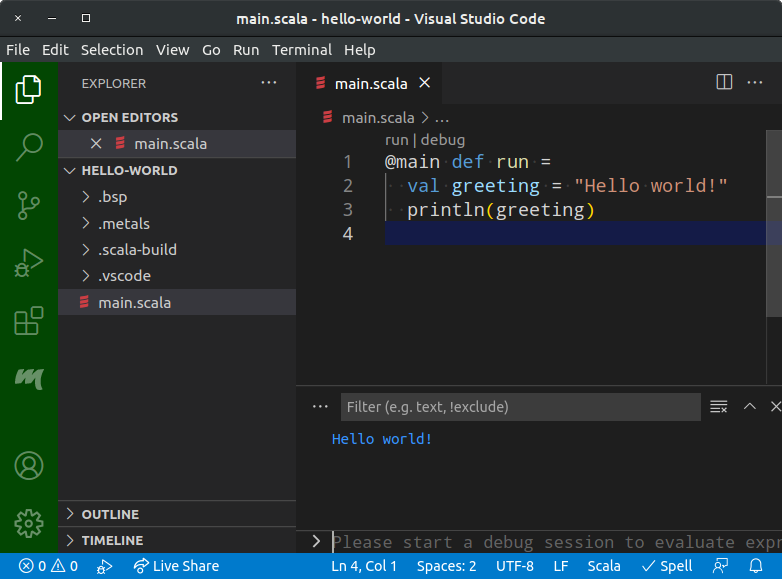
\includegraphics[width=1.0\textwidth]{../img/vscode-run}
\caption{Kör program genom att klicka på \textsf{run} ovanför huvudprogrammet. \label{appendix-ide:vscode-run}}
\end{figure}

\subsection{Köra program i VS Code}

Det finns olika sätt att köra igång huvudprogrammet i ett projekt i VS Code:

\begin{enumerate}
  \item Använd \texttt{scala-cli run .} i ett separat terminalfönster. Läs mer om \texttt{scala-cli} i Appendix \ref{appendix:compile:scala-cli}.
  \item Kör igång \texttt{sbt} i ett separat terminalfönster och kör kommandot \texttt{run} inifrån \texttt{sbt}. Detta kräver att du har en giltig \texttt{build.sbt}, se Appendix \ref{appendix:build}.
  \item Köra igång program inifrån VS Code. Detta kräver att du öppnat katalogen med din kod med File-menyns ''Open Folder'', eller genom att du startar VS Code med \texttt{code .} överst i din projektkatalog (du ser att detta är gjort om nedre meddelandefältet är blått i stället för lila). Du behöver \textit{innan} du startar VS Code en första gång köra \texttt{scala-cli setup-ide .} (se Appendix \ref{appendix:compile:scala-cli}), eller skapa en giltig \code{build.sbt}-fil (se Appendix \ref{appendix:build}) som du importerar i VS Code när frågan dyker upp i nedre högra hörnet.
  \item Kombinera Scala CLI eller \code{sbt} och VS Code. Kör detta kommando i ett separat terminalfönster: \texttt{scala-cli compile . -w}~~ där \texttt{-w} betyder \emph{watch} och gör så att ändringar bevakas. Om du istället använder \texttt{sbt} kör \code{sbt ~compile} i ett separat terminalfönster (notera tilde-tecknet som gör att ändringar bevakas). Vid ändringsbevakning kommer kompileringsfel visas där varje gång du sparar en ändring i VS Code med Ctrl+S. När alla kompileringsfel är åtgärdade och du är redo att testköra så klickar du på \textsf{run}.
\end{enumerate}

Du ser att VS Code är beredd att köra igång ditt program genom att det (efter ett tag) kommer upp en extra rad ovanför ditt huvudprogram med texten \textsf{run|debug} och då kan du klicka på \textsf{run} för att köra ditt program. Utdata från körningen visas i en flik under koden. Observera att det kan ta lite tid för VS Code att förbereda allt som behövs för att kunna köra ditt program. Håll koll på om VS Code håller på med dessa förberedelser i det blåa meddelandefältet längst ned till höger. När allt är klart efter att du startat VS Code står det ''Index complete!'' bredvid en raketsymbol i meddelandefältet.

Om något krånglar och du inte får fram \textsf{run|debug} ovanför din \code{@main}-funktion, trots du har startat VS code enligt ovan, så prova att under Metals-fliken (ikonen med det stiliserade M:et i det gröna verktygsfältet) klicka på någon av ''Restart build server'' eller ''Import build'' (den senare tar längre tid men börjar om helt) och vänta tills det står ''Index Complete!'' i det blå meddelandefältet och då ska \textsf{run|debug} synas ovanför din \code{@main}-funktion.

\begin{figure}
\centering
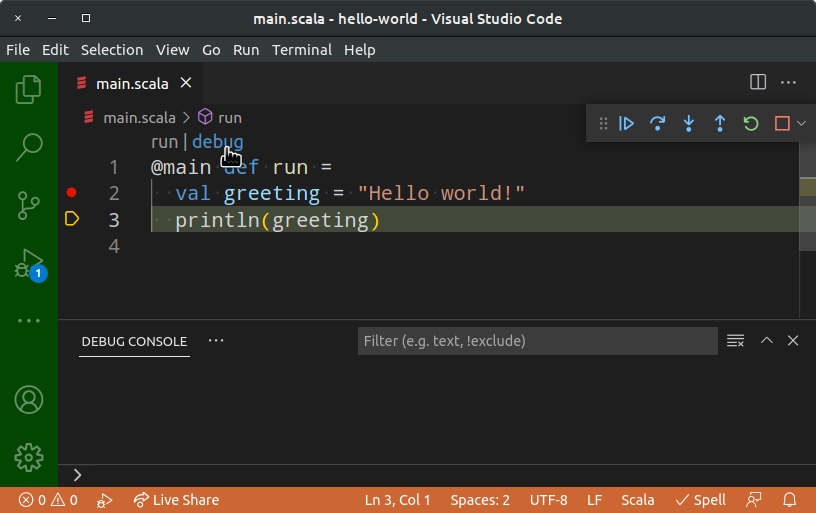
\includegraphics[width=1.0\textwidth]{../img/vscode-debug}
\caption{Debuggern i VS Code. Nederkanten är orange när debuggern kör. \label{appendix-ide:vscode-debug}}
\end{figure}

\subsection{Använda debuggern i VS Code}

Innan du börjar använda debuggern, läs först om allmän felhantering i Appendix \ref{appendix:debug}.

Du kan aktivera debuggern i VS Code för dina Scala-program genom att klicka på ''debug'' ovanför din \code{main}-metod, förutsatt att du har tillägget Metals installerad i VS Code. Du behöver även köra \texttt{scala-cli setup-ide .} en första gång (se Appendix \ref{appendix:compile:scala-cli}), eller ha en giltig \code{build.sbt}-fil (se Appendix \ref{appendix:build}) som du importerar i VS Code när frågan dyker upp i nedre högra hörnet. 

Figur \ref{appendix-ide:vscode-debug} på sidan \pageref{appendix-ide:vscode-debug} visar hur det kan se ut när debuggern i VS Code är aktiverad. När debuggern är igång får det nedersta meddelandefältet en orange färg (istället för blå). Till vänster om radnummerkolumnen kan du klicka för att aktivera och avaktivera brytpunkter. Aktiverade brytpunkter visas som en röd prick i marginalen till vänster. Den ihåliga gula pilen i marginalen pekar på den rad som kommer att exekveras härnäst. Notera panelen med olika knappar i överkanten av editorfönstret. Med dessa knappar kan du styra exekveringen enligt följande (lär dig gärna kortkommandona så blir du snabbare):
\begin{itemize}
  \item \textbf{Fortsätt}. Den blåa play-knappen kör vidare till nästa brytpunkt eller tills programmet är klart om brytpunkt ej påträffas. Kortkommando ''Continue'': F5.
  \item \textbf{Stega över}.Den blåa böjda framåtpilen kör en rad i taget \emph{utan} att hoppa in i funktioner.  Kortkommando ''Step Over'': F10.
  \item \textbf{Stega in}. Den blåa nedåtpilen kör vidare en rad i taget och hoppar in i funktioner om raden innehåller funktionsanrop. Kortkommando ''Step Into'': F11.
  \item \textbf{Stega ut}. Den blåa uppåtpilen kör klar innevarande funktion. Kortkommando ''Step Out'': Shift+F11.
  \item \textbf{Kör igen}. Den gröna återstartsikonen kör om ditt program. Kortkommando ''Restart'': Ctrl+Shift+F5.
  \item \textbf{Avbryt}. Den röda stoppknappen avbryter denna debuggingsession. Kom ihåg att avbryta innan du startar en ny debuggingsession, annars kan det lätt bli förvirrande med många samtidigt pågående körningar. Kortkommando ''Stop'': Shift+F5. 
\end{itemize}

Figur \ref{appendix-ide:vscode-trace} på sidan \pageref{appendix-ide:vscode-trace} visar hur VS Code presenterar anropsstacken och värdet på de variabler som syns där exekveringen befinner sig för tillfället. Du får fram detta genom att klicka på ikonen med en lus och en playknapp i det vertikala, gröna verktygsfältet längst till vänster. I en blå ring står en etta om du har startat en debuggingsession. Om det står en tvåa eller mer så har du flera sessioner igång och då kan det vara klokt att avsluta alla utom en, så att inte förvirring uppstår om vilken session som är den aktuella. 

\begin{figure}
\centering
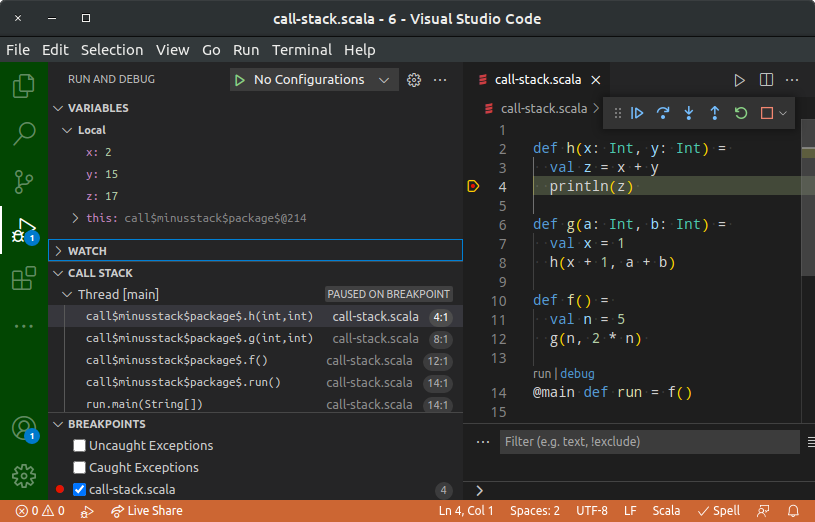
\includegraphics[width=1.0\textwidth]{../img/vscode-trace}
\caption{Anropsstack och variabler i VS Code.\label{appendix-ide:vscode-trace}}
\end{figure}

Mycket av konsten i debugging handlar om att undersöka variablers värde under exekveringen för att ta reda på om din hypotes om vad som händer under exekvering verkligen stämmer, eller om något egentligen inte fungerar så som du antar. Detta kan du med fördel göra genom att placera brytpunkter på relevanta ställen. Även vid användning av en debugger kan du ha stor nytta av att göra \code{println} av intressanta uttryck för att i detalj undersöka vad som egentligen händer. Läs mer om debugging i Appendix \ref{appendix:debug}.
 